%%%%%%%%%%%%%%%%%%%%%%%%%%%%%%%%%%%
% Chatbot
%%%%%%%%%%%%%%%%%%%%%%%%%%%%%%%%%%%
\section{Chatbot}
In previous sections we have concluded that teachers do not have the time and resources they need to academically lift their students as high as possible. One way of fixing this issue could be through the use of a chatbot, one that could help the students by answering easier questions and notifying the teacher of the needs of their students. Therefore this section will highlight what chatbots are and how they can be used to combat the issue. 
\newline\newline
Furthermore the section will explain some of the core elements of a chatbot and its functions. It will also cover what features a chatbot is expected to have.
The chapter will also cover some of the current chatbots that are in use today, and then give an explanation of the essential concept
\newacr{Natural Language Processing}{NLP}.

%%%%%%%%%%%%%%%%%%%%%%%%%%%
% What is a chatbot?
%%%%%%%%%%%%%%%%%%%%%%%%%%%
\subsection{What is a chatbot?}
A chatbot is a computer program designed to simulate conversation with human users. Chatbots can be used for various tasks in today's society, everything from working as an assistant for customer support on various websites \cite{OlgaVeretskaya2017WhatAnadea} to acting as a companion for seniors or people with Alzheimer's in order to help with their loneliness \cite{GeorgefomitchevChatBotsEnduranceRobots}.
\newline\newline 
The first chatbot was created from 1964 to 1966 at the MIT Artificial intelligence Laboratory by the German American computer scientist Joseph Weizenbaum. He gave the chatbot the name ELIZA. It was made as an early NLP computer build for demonstrating the superficiality of communications between humans and machines. ELIZA communicated with humans by simulating conversations using pattern matching \cite{ELIZAWikipedia}. Pattern matching is when a computer checks a given sequence of tokens for patterns and responds with a predetermined response that correlates to that specific pattern of tokens \cite{Warth2007OMeta:}. This gave some users the impression that they were talking to a real human-being rather than a computer program. ELIZA did however fail the Turing Test \cite{ELIZAWikipedia}. The Turing Test, also known as "The imitation Game", was first proposed by Alan Turing in 1951 and was made to settle the issue of a machines intelligence \cite{Psych.utorontoArtificialTest}.

%%%%%%%%%%%%%%%%%%%%%%%%%%%
% Good Features
%%%%%%%%%%%%%%%%%%%%%%%%%%%
\subsection{Different chatbot features}
Chatbots nowadays are very different from when ELIZA was first created. The digital world is expanding with rapid speed. This makes the users expectations of chatbots much higher and they expect a better, more interactive experience with chatbots.
Companies are competing against each other to provide the best customer experience. The digital world of customer service is being redefined by the use of AI and chatbots.
For a chatbot to give the user a good experience, it needs to have different features. There are many features a chatbot can use, but there are some that are more prioritized when it comes to the user interaction as described below.

%%%%%%%%%%%%%%%%%%%%%
% Conversational maturity
%%%%%%%%%%%%%%%%%%%%%
\begin{itemize}
    \item \textbf{Conversational maturity} is when a chatbot has the ability to understand more and interact conversationally with the user. Chatbots need the capability to understand the context of a conversation through specific NLP. The use of NLP will make the chatbot interact with the user in a more human-like way, which would make it more likely that the user thinks they are talking to a person rather than a chatbot.The use of NLP will make the chatbot smarter, and allow it to suggest options based on the users preference \cite{MayaS2017TopNewlands}. The project will go further into explaining the concept of NLP in section \ref{subsub:natural_language_processing} .
    \newline
    A chatbot also needs to have the ability to read the intent of a question and what is being sought by the user, so it can give the user an accurate first response. One way to approach this is to make use of proposing options to clarify or confirm the users intent. A good chatbot has the capability of proactively seeking out information giving it a more advanced conversational capability \cite{Furniss20177Chatbot}.
    
    \item A \textbf{Freely exploring} chatbot is able to freely explore information. It would be able to reach, consume, and process vast amounts of data both structured and unstructured to surface insights from any source.
    This would make the chatbot able to clarify questions, even if the user has not fully clarified the intent or holding a linear conversation with the it \cite{Furniss20177Chatbot}.
    
    \item \textbf{Omni-caple}, a good chatbot will be able to retain data and context over different conversations with the same user. This will help it to keep the conversation seamless and make a good experience with the user \cite{Furniss20177Chatbot}.
    
    \item \textbf{Emotional intelligence} makes the chatbot able  to infer the user's personality traits and understand their sentiment and tone. It would therefore be able to give the user a personalized experience \cite{Furniss20177Chatbot}.
    
    \item \textbf{Autonomous reasoning} allows the chatbot to perform certain reasoning without the intervention from a human. Through NLP it would use past case histories to come up with a specific solution for the user \cite{Furniss20177Chatbot}.
\end{itemize}

%%%%%%%%%%%%%%%%%%%%%
% Natural Language Processing
%%%%%%%%%%%%%%%%%%%%%
\subsection{Natural Language Processing}
\label{subsub:natural_language_processing}
\newacr{Natural Language Processing}{NLP} is a sub-field of \newacr{Artificial Intelligence}{AI} that focuses on enabling computers to understand and process human languages in order to get computers closer to a human-level understanding of language.
\newline\newline
Computers are great at understanding standardised and structured data like database tables and financial records and they are able to process the data much faster than humans can \cite{Seif2018AnProcessing}. 
%There is just one problem. Humans do not communicate in \enquote{structured data} or speak binary .
\newline\newline
There are no standardised techniques for the computer to process natural language. When using programming languages we are essentially giving the computer a set of rules that it should operate by. With unstructured data, these rules are quite abstract and challenging to define \cite{Seif2018AnProcessing}.
\newline\newline
What makes NLP hard is that some words mean different things in different contexts. For example, something being on fire could mean literally being on fire or it could also be a metaphor for being really good at something. Humans understand this but computers cannot contextualize sentences \cite{Seif2018AnProcessing}.
\newline\newline
When using NLP, you can start by doing a basic thing called tokenization, where you split a text into phrases, words, numbers, identifiers or punctuation \cite{NelsonNaturalTechnologies}. After this you can do an entity analysis. You go through a text to identify all the important words or \enquote{entities}. Where \enquote{important} means words that have some kind of real-world semantic meaning or significance \cite{NelsonNaturalTechnologies}. On \figureref{fig:EntityAnalysis} you can see an example of how the analysis works.

\begin{figure}[H]
    \centering
    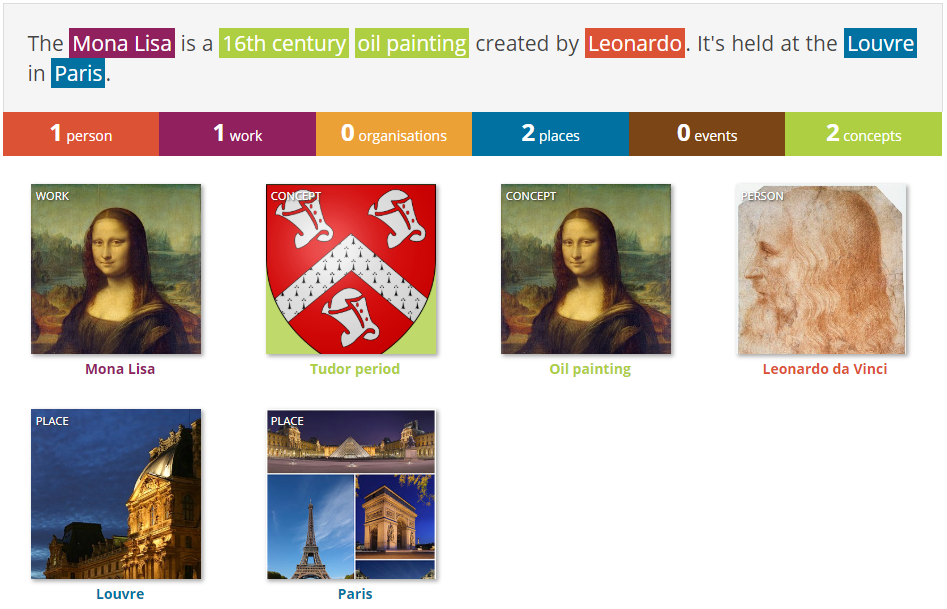
\includegraphics[width=0.6\textwidth]{figures/EntityAnalysis.png}
    \caption{Example of an entity analysis \cite{DemoAPI}}
    \label{fig:EntityAnalysis}
\end{figure}

\noindent
After using an entity analysis you can extract the most important phrases from a text by using the two techniques below \cite{NelsonNaturalTechnologies}:

\begin{itemize}
    \item \textbf{Part of speech tagging} allows you to identity phrases from noun or verb clauses.
    \item \textbf{Statistical phrase extraction} is used to identify token sequences which occur more frequently than expected by chance.
\end{itemize}

\noindent
Another thing you can use is semantics analysis. It is used to extract the subjective meaning from a text to perform a sentiment analysis where you can determine the \enquote{attitude} of a single word or a collection of words. You can use this on social media sites like Facebook or Twitter to identify trends of a public opinion by looking at how often a word appears in a specific context to interpret the tone in a discussion \cite{Plapinger2017AScience}.

%%%%%%%%%%%%%%%%%%%%%%%%%%%
% The use of chatbots
%%%%%%%%%%%%%%%%%%%%%%%%%%%
\subsection{The use of chatbots}
The use of an AI efficient teaching assistant would be able to help teachers making sure the students would get the help they need \cite{Singh2018AIFutureHold}.
As mentioned in section \ref{sec:teacher_workload} with the amount of students in each class the teacher can not come around to every student and as a result they do not have the time to tend the needs of all their students.
\newline\newline
A chatbot would make it possible to connect to the whole class through the use of AI. Chatbots with artificial intelligence technology would have the ability to teach student the necessary lecture by turning the lecture into a series of messages. This would make it easy for the student to find the necessary information about the assignments given by the teacher.
The current generation of student is already integrated with technology in their daily life and is used to get everything instantly, whether it is sending pictures, sending emails or even finding help with their assignments online \cite{Singh2018AIFutureHold}. 
\newline\noindent
A chatbot would be able to help a student with their courses with the necessary information. If a student would get in trouble with a certain subject the student would be able with the use of the chatbot to instantly get the help needed \cite{Singh2018AIFutureHold}.
\newline\newline
This would benefit both the teachers using the chatbot to make sure all students would get the help needed.
By making sure the students would get the help needed instantly and not having to wait on the teacher to assist them, which is specially a problem in bigger classrooms. The students would be able to get the information on how to solve the assignment instantly \cite{Gibori2012TheStudents}.

%%%%%%%%%%%%%%%%%%%%%%%%%%%
% Existing Solutions
%%%%%%%%%%%%%%%%%%%%%%%%%%%
\subsection{Existing Solutions}
\label{sub:Existing Solutions}
The report is focusing on teaching in the subject of math and there are already some chatbots targeting this area. Some of the chatbots are working as plugins in already existing applications such as Discord \cite{DiscordDownloads} and Messenger \cite{Messenger} but there are also academic projects that is using more sophisticated bots. In \tableref{table:a_list_of_solution_features} there is listed the solutions' features.

\setlength{\tabcolsep}{0.5em} % for the horizontal padding
\renewcommand{\arraystretch}{1.5}% for the vertical padding
\definecolor{lightgray}{rgb}{0.95, 0.95, 0.95}
\rowcolors{2}{lightgray}{white}
\begin{table}[H]
\centering
\small
\begin{tabular}{|l|c|c|c|}
\hline
\rowcolor[HTML]{FFFFFF} 
\multicolumn{1}{|c|}{\cellcolor[HTML]{FFFFFF}{\color[HTML]{000000}\backslashbox[135pt][l]{Features}{Solutions}}} & \multicolumn{1}{c|}{\cellcolor[HTML]{FFFFFF}{\color[HTML]{000000} MathBot}} & \multicolumn{1}{c|}{\cellcolor[HTML]{FFFFFF}{\color[HTML]{000000} Miao}} & \multicolumn{1}{c|}{\cellcolor[HTML]{FFFFFF}{\color[HTML]{000000} Sofia}} \\ 
\hline
Simple calculator               & X & X & X \\ 
\hline
Advanced calculator             & X & X & X \\
\hline
LaTeX integration               & X & - & X \\
\hline
Topic learning                  & - & X & X \\ 
\hline
Can learn from the user         & - & - & X \\ 
\hline
Personal assistent integration  & - & X & X \\ 
\hline
\end{tabular}%
    \caption{A list of solution features}
    \label{table:a_list_of_solution_features}
\end{table}

\noindent
One of the solutions is MathBot, which is a bot you can add to your Discord server \cite{MathBotBots}. The bot is then working as a calculator that can solve simple math or you can write more advanced problems in the LaTex format. It also includes some small features like a randomizer, where you can ask to get a number between zero and the number you gave as an input. 
\newline\newline
Within Messenger you can use the bot Miao that helps you with different kinds of Math and Science concepts but it can also solve more advanced equations \cite{MiaoAcademy}. You can ask the bot questions like \textit{How to prove similar triangles?} and it will then give you a short answer together with some resources where you can learn more about the concept \cite{MiaoAcademy}.
\newline\newline
An academic project at Harvard \cite{KnillAnEducation} around the topic of an artificial intelligence experiment in college math education sought to shed light on basic questions in education such as:
\begin{itemize}
    \item How do we teach effectively?
    \item How do students learn?
\end{itemize}
\noindent
To help gather information they developed an AI tool called \enquote{Sofia} to help students with calculus and related issues. The bot uses a simple chat interface to communicate with the user. The bot works as a calculator where you can both give it an equation but you can also write the command in natural language:
\begin{itemize}
    \item \textbf{{\footnotesize \enquote{find lagrange solution x\^{}2+y\^{}2+y and 4x-5x\^{}2-y\^{}2-3*y-3}}}
    \item \textbf{{\footnotesize \enquote{add three and four and seven}}}
\end{itemize}
\noindent
You can also ask the bot questions about math but it can also answer questions where you normally would use either Google Assistant or Siri \cite{GoogleGoogle}\cite{SiriApple}. Below you can see some examples of the questions you can ask:
\begin{itemize}
    \item \textbf{{\footnotesize \enquote{what is the weather}}}
    \item \textbf{{\footnotesize \enquote{what is a determinant}}}
\end{itemize}

%\subsubsection{Advantages & Disadvantages}

\begin{comment}
% MathBot
% Advantages
1. Functions in an already working environment so the users are already used to the user interface
2. Simple interface
3. LaTeX integration
4. Advanced calculator
% Disadvantages
1. Functions only as an advanced calculator you can not get help for specific topics

% Miao
% Advantages
1. Functions in an already working environment so the users are already used to the user interface
2. Simple interface
3. Can help with a wide range of math topics

% Disadvantages


% Sofia
% Advantages
1. Can learn from the user
2. LaTeX integration
3. Advanced calculator

% Disadvantages
1. Can only help with topics related to calculus

\end{comment}






